\documentclass[ignorenonframetext,]{beamer}
\usetheme{Szeged}
\usecolortheme{sidebartab}
\usefonttheme{professionalfonts}


\usepackage{amssymb,amsmath}
\usepackage{ifxetex,ifluatex}
\usepackage{fixltx2e} % provides \textsubscript
\usepackage{lmodern}
\ifxetex
  \usepackage{fontspec,xltxtra,xunicode}
  \usepackage[cjk,hangul]{kotex}
  \defaultfontfeatures{Mapping=tex-text,Scale=MatchLowercase}
  \newcommand{\euro}{€}
\else
  \ifluatex
    \usepackage{fontspec}
    \defaultfontfeatures{Mapping=tex-text,Scale=MatchLowercase}
    \newcommand{\euro}{€}
  \else
    \usepackage[T1]{fontenc}
    \usepackage[utf8]{inputenc}
    \usepackage[cjk,hangul]{kotex}
      \fi
\fi
\IfFileExists{upquote.sty}{\usepackage{upquote}}{}
% use microtype if available
\IfFileExists{microtype.sty}{\usepackage{microtype}}{}
\usepackage{url}
\usepackage{letltxmacro}
\makeatletter
\def\maxwidth{\ifdim\Gin@nat@width>\linewidth\linewidth\else\Gin@nat@width\fi}
\def\maxheight{\ifdim\Gin@nat@height>\textheight0.8\textheight\else\Gin@nat@height\fi}
\makeatother
\AtBeginDocument{
  \LetLtxMacro\Oldincludegraphics\includegraphics
  \renewcommand{\includegraphics}[2][]{%
    \Oldincludegraphics[#1,width=\maxwidth,height=\maxheight,keepaspectratio]{#2}}
}

% Comment these out if you don't want a slide with just the
% part/section/subsection/subsubsection title:
\AtBeginPart{
  \let\insertpartnumber\relax
  \let\partname\relax
  \frame{\partpage}
}
\AtBeginSection{
  \let\insertsectionnumber\relax
  \let\sectionname\relax
  \frame{\sectionpage}
}
\AtBeginSubsection{
  \let\insertsubsectionnumber\relax
  \let\subsectionname\relax
  \frame{\subsectionpage}
}

\setlength{\parindent}{0pt}
\setlength{\parskip}{6pt plus 2pt minus 1pt}
\setlength{\emergencystretch}{3em}  % prevent overfull lines
\setcounter{secnumdepth}{0}

\title{Bayesian Inference using Opinion Survey of Seoul Mayoral Election}
\author{Computer Science Dep. 전희원}
\date{2014-06-23}

\begin{document}
\frame{\titlepage}

\begin{frame}{Background}

\begin{quote}
Bayesian had been used on election result prediction effectively. Most
recent prediction was done by \texttt{Nate Silver} in the 2012 United
States presidential election(he correctly predicted the winner of all 50
states). Formaly, John W.Tukey was projecting the election-day results
of presidential contests for national television.
\end{quote}

\end{frame}

\begin{frame}{Purpose}

\begin{itemize}
\itemsep1pt\parskip0pt\parsep0pt
\item
  Estimate support ratio differences of two candidates using
  \texttt{6.4} Seoul mayoral election.
\item
  Compare result between frequentist and bayesian method.
\item
  Compare \texttt{6.4} result with bayesian estimation.
\end{itemize}

\end{frame}

\begin{frame}{Data}

\begin{itemize}
\itemsep1pt\parskip0pt\parsep0pt
\item
  Data : National Election Commission \url{https://www.nesdc.go.kr}
\item
  Range : \texttt{2014-03-24} \textasciitilde{} \texttt{2014-05-28}
\item
  \texttt{\#} of Survey : 31
\item
  \texttt{\#} of Survey Orgs. : 16
\item
  \texttt{\#} of Request Orgs. : 21
\end{itemize}

\end{frame}

\begin{frame}{EDA}

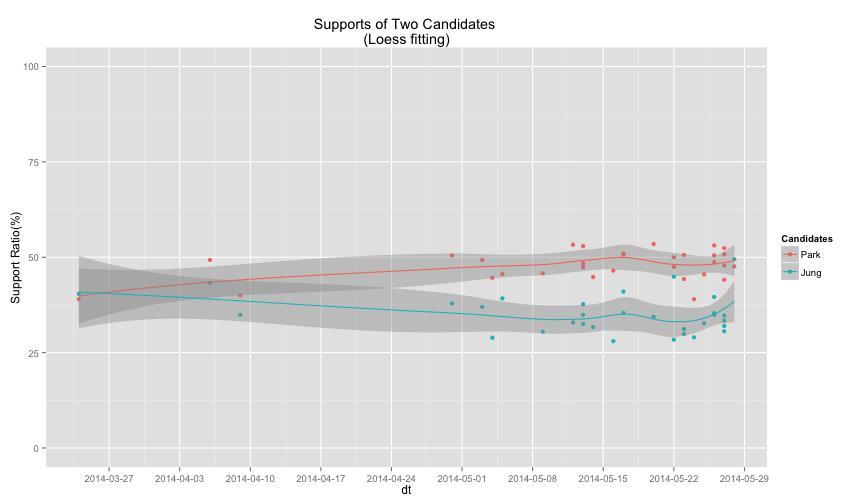
\includegraphics{./presentation_files/figure-beamer/eda.png}

\end{frame}

\begin{frame}{Multinomial Likelihood with a Dirichlet Prior}

\begin{itemize}
\itemsep1pt\parskip0pt\parsep0pt
\item
  Support Counts(j :Jung , p :Park, e :Etc.)

  \begin{itemize}
  \itemsep1pt\parskip0pt\parsep0pt
  \item
    $n_j, n_p, n_e$
  \end{itemize}
\item
  Likelihood

  \begin{itemize}
  \itemsep1pt\parskip0pt\parsep0pt
  \item
    $X_j,X_p,X_e \sim Multinomial(n, \theta_{n_j}, \theta_{n_p}, \theta_{n_e})$
  \end{itemize}
\item
  Prior

  \begin{itemize}
  \itemsep1pt\parskip0pt\parsep0pt
  \item
    $\pi(\theta_j, \theta_p, \theta_e) \propto 1$
  \item
    $\theta_{n_j}, \theta_{n_p}, \theta_{n_e} \sim Dirichlet(1,1,1)$
  \end{itemize}
\item
  Posterior

  \begin{itemize}
  \itemsep1pt\parskip0pt\parsep0pt
  \item
    $\theta_{n_j}, \theta_{n_p}, \theta_{n_e}|n_j,n_p,n_e \sim Dirichlet(n_j + 1, n_p + 1, n_e + 1)$
  \end{itemize}
\end{itemize}

\end{frame}

\begin{frame}{Steps}

\begin{enumerate}
\def\labelenumi{\arabic{enumi}.}
\itemsep1pt\parskip0pt\parsep0pt
\item
  Set uniform prior
\item
  Update posterior distribution parameters on each survey.
\item
  Do Monte Carlo Simulation and get samples on each parameters(10,000
  samples).
\item
  Get $\theta_p - \theta_j$ distribution and mean of that.
\end{enumerate}

\end{frame}

\begin{frame}{Mean of Posterior}

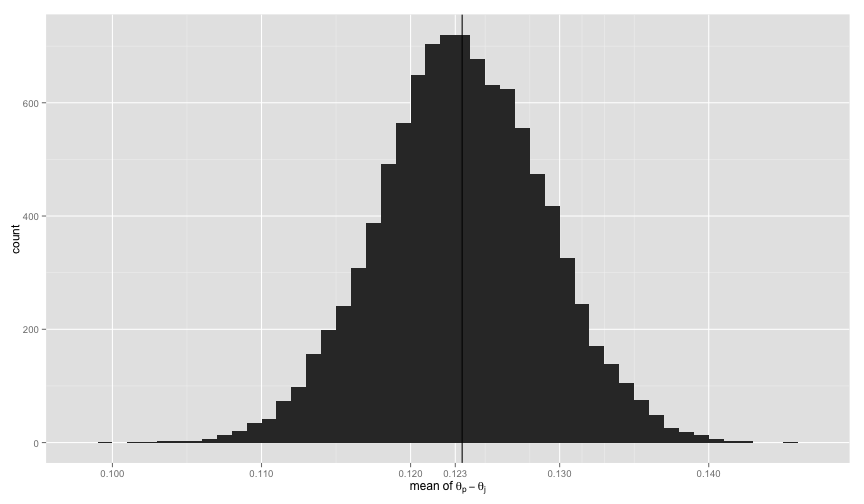
\includegraphics{./presentation_files/figure-beamer/mc.png}

\end{frame}

\begin{frame}{Comparison between Frequentist and Bayesian}

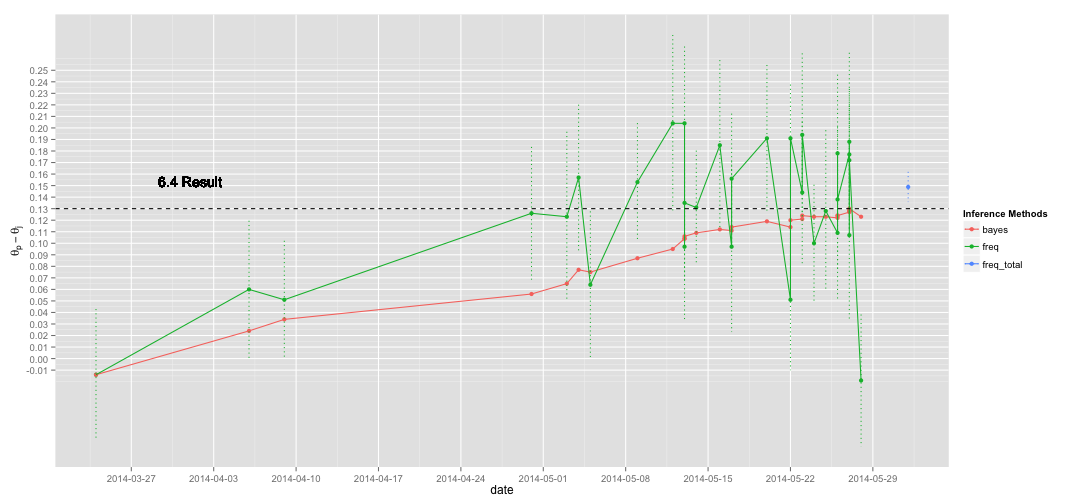
\includegraphics{./presentation_files/figure-beamer/comp.png}

\end{frame}

\begin{frame}{Conclusion}

\begin{itemize}
\itemsep1pt\parskip0pt\parsep0pt
\item
  Bayesian results quite good(0.0066 error).
\item
  \texttt{0\%} error when exclude abnormal survey on
  \texttt{2014-05-28}.
\end{itemize}

\end{frame}

\begin{frame}{References}

\begin{itemize}
\itemsep1pt\parskip0pt\parsep0pt
\item
  Gelman, et. al. Bayesian Data Analysis 3nd (2013, p.~69)
\item
  Andrew D. Martin, Kevin M. Quinn, Jong Hee Park (2011). MCMCpack:
  Markov Chain Monte Carlo in R. Journal of Statistical Software. 42(9):
  1-21. URL \url{http://www.jstatsoft.org/v42/i09/}.
\end{itemize}

\end{frame}

\end{document}
